\chapter{Simulation}
This section of the report describes the testing of separate signal processing steps in a simulated environment. Each block as seen in Figure~\ref{fig:global_thesis_flowchart} will be tested individually, and the method and results will be discussion on a per-block basis:
\begin{itemize}
    \item Pre-whitening
    \item Filtering
    \item Envelope estimation
\end{itemize}

Unless specified otherwise all signals will be high-passed with an $f_\text{cut}$ of \SI{1}{\hertz} to remove DC bias before any operation is applied

\section{Pre-whitening}\label{sec:whitening}
A whitening filter is a digital filter with a frequency response that is (ideally) the inverse of the frequency contents of an sEMG signal. 

\subsection{Method}
A testing signal was created that approximates the frequency response of an sEMG signal. The testing signal was created by creating a long white noise signal and multiplying the amplitudes in the frequency spectrum with a curve that estimates the frequency response of an sEMG signal. After this the signal is passed through inverse fft to go back to a time-domain signal. The result can be seen in \ref{fig:whitening_simulation} subplot 1 and 2.

The whitening filter is then created by taking the FFT of the time-domain test signal and taking its reciprocal at every frequency. Lastly the whitening filter frequencies are multiplied by the mean of the original signal frequencies to make sure that when the filter is applied the mean stays the same. These steps can be seen in \ref{fig:whitening_simulation} subplot 3. 

\subsection{Results}
\begin{figure}[h!t]
	\begin{center}
		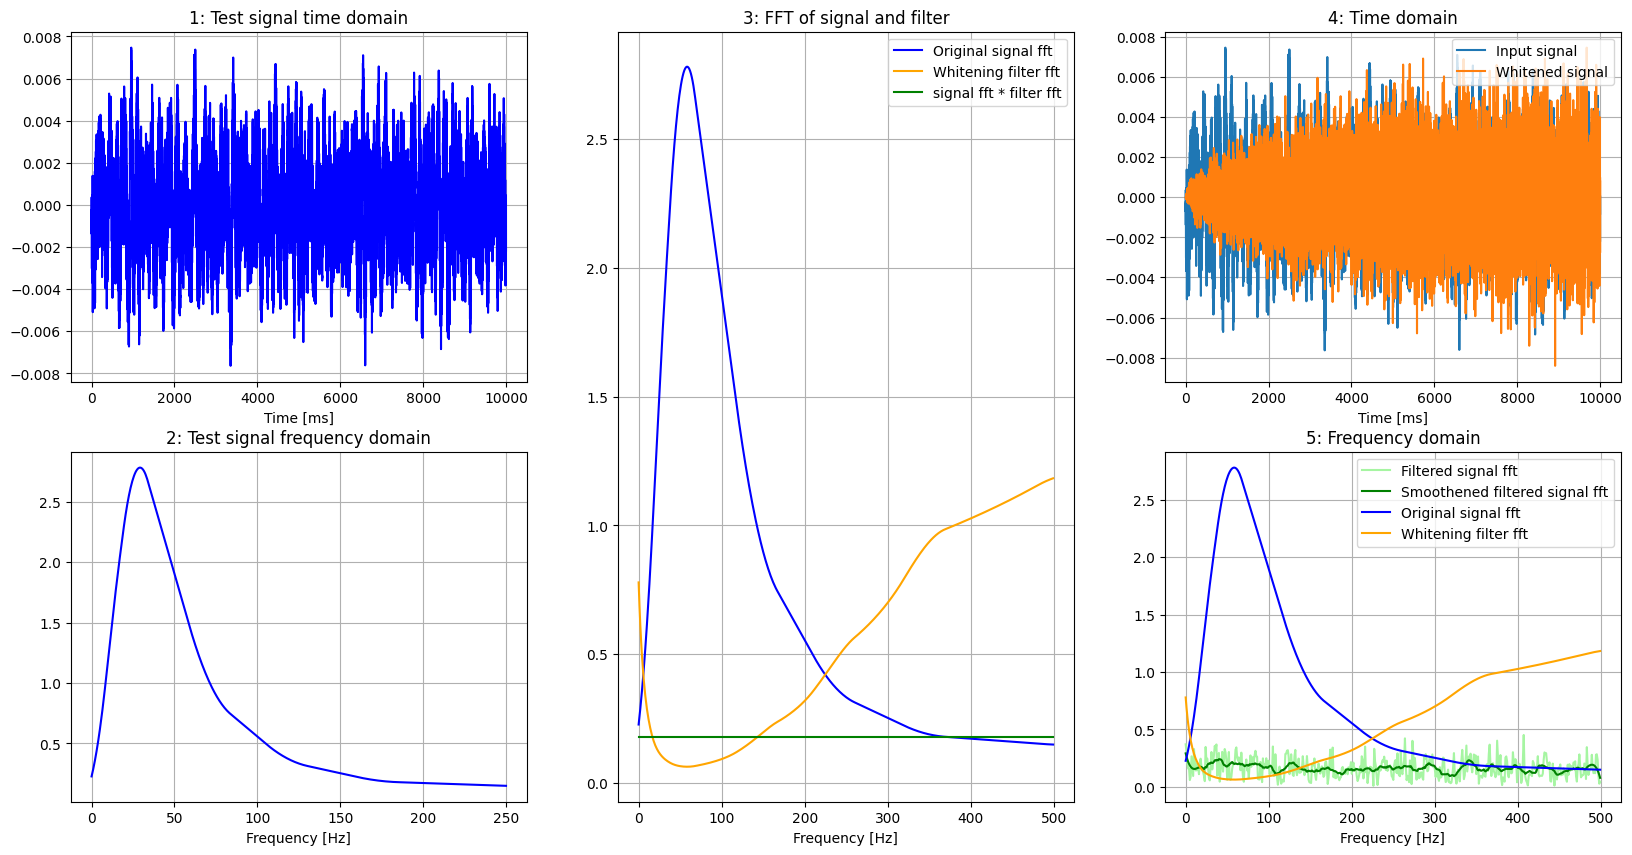
\includegraphics[width=1.0\columnwidth]{images/prewhitening_simulation.png}
	\end{center}
	\caption{Subplot 1 and 2 display the input simulated input signal with a frequency response that approximates the frequency contents of an sEMG signal. Subplot 3 displays the frequency content of the signal, the subsequently calculated whitening filter, and the multiplication of the signal with the filter in frequency domain to show that the response is indeed white. Subplot 4 and 5 show the original and 'whitened' signal in time domain and frequency domain.}
	\label{fig:whitening_simulation}
\end{figure}

Figure~\ref{fig:whitening_simulation} shows the whitening filter that functions as expected. In the center subplot the 'ideal' result are shown (multiplication in the frequency domain), and in subplot 5 the result from convolution in the time domain is shown. In subplot 5 a smoothed version of the filtered signal FFT is added to display that the signal power has a mean that approximates white noise. This filter was made using a Savitzky-Golay filter with a window length of 31 and a polynomial order of 3.

\section{Filtering}
First the metrics are introduced that will be used to compare filter performance. Subsequently, the construction process of each filter is presented. Lastly the different filtering methods are compared.

\subsection{Comparison metrics}
Each filter will be tested using two metrics: SNR (eq \ref{eq:snr}) and Bandwidth (definition of this will be given shortly). All filters are linear time invariant which means the superposition principle can be used to simplify SNR calculations \cite{linear_systems_theory}. The superposition principle simply states that filtering the sum of two signals is the same as filtering the signals individually and adding the results. An illustration of this can be seen in \ref{fig:filter_process}. 

Due to the difficulty of creating a simulated signal that has the frequency contents of an sEMG signal and environmental noise, a pre-recorded sample of sEMG of a bicep going through maximum voluntary contraction was used to test the filters. This sample is not used for force estimation because it will not be compared to the contraction of an antagonistic muscle and purely the frequency contents of the signal are of interest. The sample that is used can be seen in Figure~\ref{fig:sEMG_signal_example}. Noise is taken to be \SIrange{0}{2}{\second} and signal is taken to be \SIrange{5}{7}{\second}. The RMS of the filtered signal is divided by the RMS of the filtered noise to create a signal to noise ratio.

\begin{figure}[h!t]
	\begin{center}
		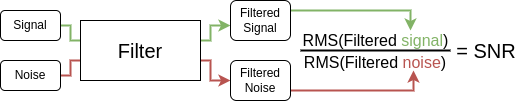
\includegraphics[width=1.0\columnwidth]{images/filter_process.png}
	\end{center}
	\caption{Illustration of testing of filters. Signal and noise are passed through the filter individually and the SNR is calculated for each filter.}
	\label{fig:filter_process}
\end{figure}

SNR by itself is not a valid metric for judging a filters performance in this scenario. The purpose of improving SNR is the assumption that force can be estimated more accurately from a signal that contains primarily the signal generated by muscle contraction. However, a filter may be able to attenuate the signal and noise in such a way that the SNR is very high, but the signal is attenuated to such a degree that it no longer resembles the original signal that was generated by the muscle contraction. An example of this can be seen in Figure~\ref{fig:good_snr_bad_integrity}. 

A measure to define how much the frequency spectrum has changed is the bandwidth. Typically the bandwidth of a signal is defined as the range of frequencies between two frequency points outside of which the signal is attenuated more than a specific threshold value \cite{bandwidth_definition}. This definition is not applicable to this problem as the frequencies that are 'present' in an sEMG signal are not necessarily consecutive. Therefore the bandwidth of an sEMG signal will be defined as the number of frequency components that are larger than the mean of the frequency spectrum, a mathematical definition is given in Equation~\ref{eq:bandwidth}. With this metric, a frequency spectrum such as the one seen in Figure~\ref{fig:good_snr_bad_integrity} will have a low bandwidth because most frequencies are below the mean.

\begin{equation}\label{eq:bandwidth}
    \text{Bandwidth} = \# \{x\in \text{fft(sig)} \mid x> \overline{\text{fft(sig)}}\} 
\end{equation}

\begin{figure}[h!t]
	\begin{center}
		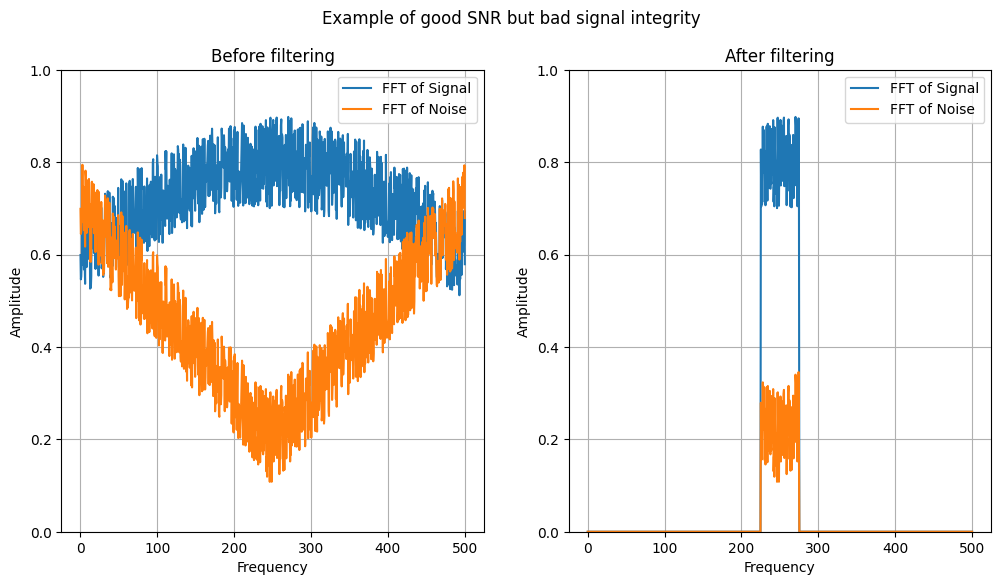
\includegraphics[width=1.0\columnwidth]{images/good_snr_bad_integrity.png}
	\end{center}
	\caption{Example of filtering that results in good SNR but bad bandwidth.}
	\label{fig:good_snr_bad_integrity}
\end{figure}


\subsection{Method}
\subsubsection{Static filter}
The theory from section \ref{section:standard_semg_processing} specifies the removal of DC frequencies, a notch filter at \SI{50}{Hz}, and a bandpass filter between \SI{20}{Hz} and \SI{300}{Hz}. Looking at the noise spectrum in Figure~\ref{fig:sEMG_fft_signalnoise_example} it can be seen that there also exist significant peaks at \SI{100}{Hz} and \SI{150}{Hz}. Therefore different static filters were tested with different amounts of notch filters. 

\begin{itemize}
    \item IIR Notch filters at \SI{50}{Hz}, \SI{100}{Hz}, \SI{150}{Hz}, \SI{200}{Hz}. All have a Q-factor of 10, are constructed as numerator/denominator pairs and applied using scipy's lfilter.
    \item The bandpass filter consists of a high-pass filter with an $f_\text{cut}$ of \SI{20}{Hz} and a lowpass filter with an $f_\text{cut}$ of \SI{300}{Hz}. Both filters are of length 5, are constructed as numerator/denominator pairs, and applied using scipy's lfilter.
\end{itemize}

The frequency response of these filters can be seen in Figure~\ref{fig:staticfilter_notches_frequencyresponse}. The resulting metrics can be seen in the chart \ref{fig:staticfilter_notches_barchart}.

\begin{figure}[h!t]
	\begin{center}
		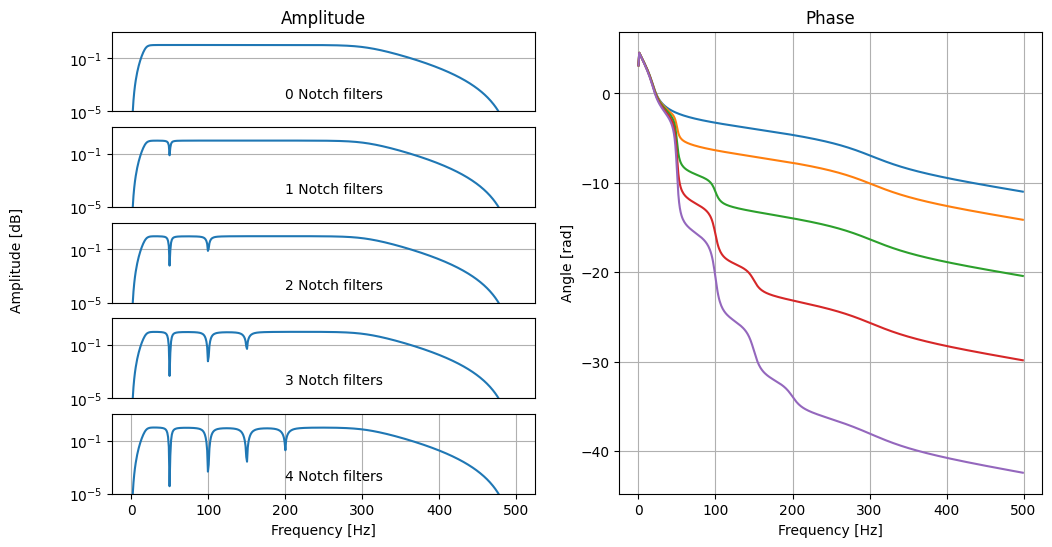
\includegraphics[width=1.0\columnwidth]{images/staticfilter_notches_frequencyresponse.png}
	\end{center}
	\caption{Frequency response of static filters with a different number of notch filters. The plots were created by determining the frequency responses of each individual filter (notches, low-pass, high-pass), then multiplying the amplitudes and adding the phase shifts. For the sake of illustration the amplitude graphs have been shifted vertically to clearly show the existence of notch filters in different lines, during simulations this shift was not present. }
	\label{fig:staticfilter_notches_frequencyresponse}
\end{figure}

\begin{figure}[h!t]
	\begin{center}
		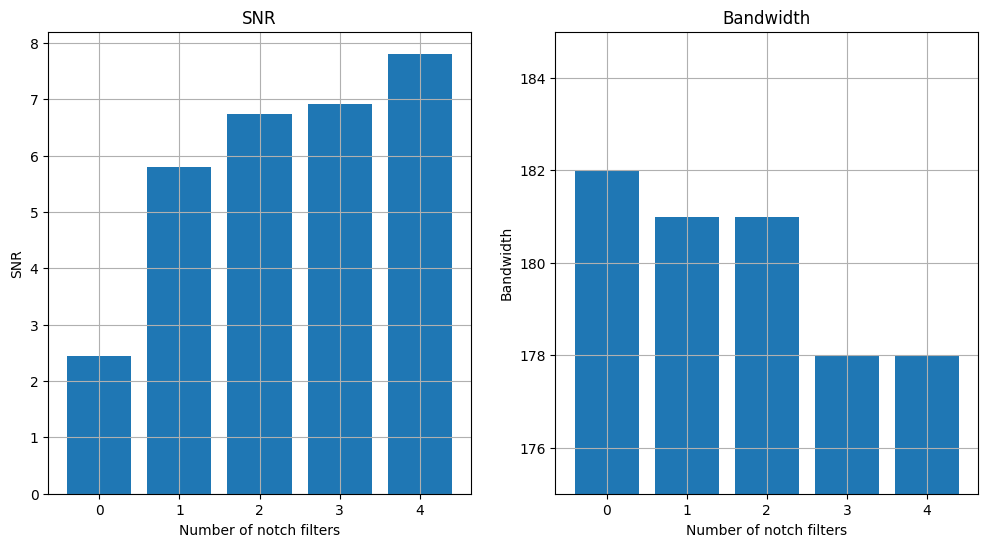
\includegraphics[width=1.0\columnwidth]{images/staticfilter_notches_barchart.png}
	\end{center}
	\caption{SNR and bandwidth of static filters with different numbers of Notch filters. Three notch filters were chosen for the measurement section (\ref{sec:measurements}) as the bandwidth seems to not depend very much on number of filters but in Figure~\ref{fig:sEMG_fft_signalnoise_example} the peak around \SI{200}{\hertz} is insignificant compared to other multiples of \SI{50}{\hertz}}
	\label{fig:staticfilter_notches_barchart}
\end{figure}


\subsubsection{Wiener filter}
As discussed in section \ref{sec:filters_theory} the Wiener filter coefficients are constructed from the cross-correlation vector between signal+noise ($d(n)$) and the noise ($v(n)$) and the auto-correlation of the noise as is presented in the Wiener-Hopf equation in Equation~\ref{eq:wiener_hopf} \cite{lecture_adaptive_filters_1}. 

\begin{equation}
    w_\text{opt} = R^{-1}P
    \label{eq:wiener_hopf}
\end{equation}

The number of Wiener filter coefficients have a strong influence on the performance of the filter as can be seen in Figure~\ref{fig:wiener_filter_length}. For the measurements section (\ref{sec:measurements}), a Wiener filter of length 500 was chosen as this is a middle ground for SNR and bandwidth.

\begin{figure}[h!t]
	\begin{center}
		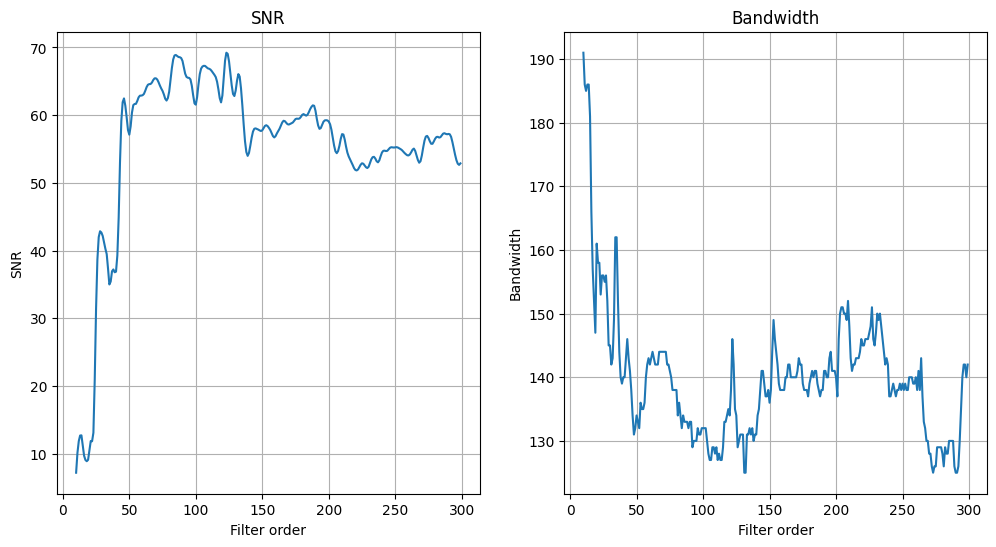
\includegraphics[width=1.0\columnwidth]{images/wiener_filter_length.png}
	\end{center}
	\caption{The effect of the number of Wiener filter coefficients on the SNR and bandwidth. To clarify the more general influence of filter length both plots were smoothed using a Savitzky-Golay filter with length of 71 and poly order of 3. It appears there is a clear peak in SNR at 650 filter terms but this corresponds to a low bandwidth. A filter length of 500 was chosen as this presents a good middle ground between SNR and bandwidth peak in the bandwidth. }
	\label{fig:wiener_filter_length}
\end{figure}

\begin{figure}[h!t]
	\begin{center}
		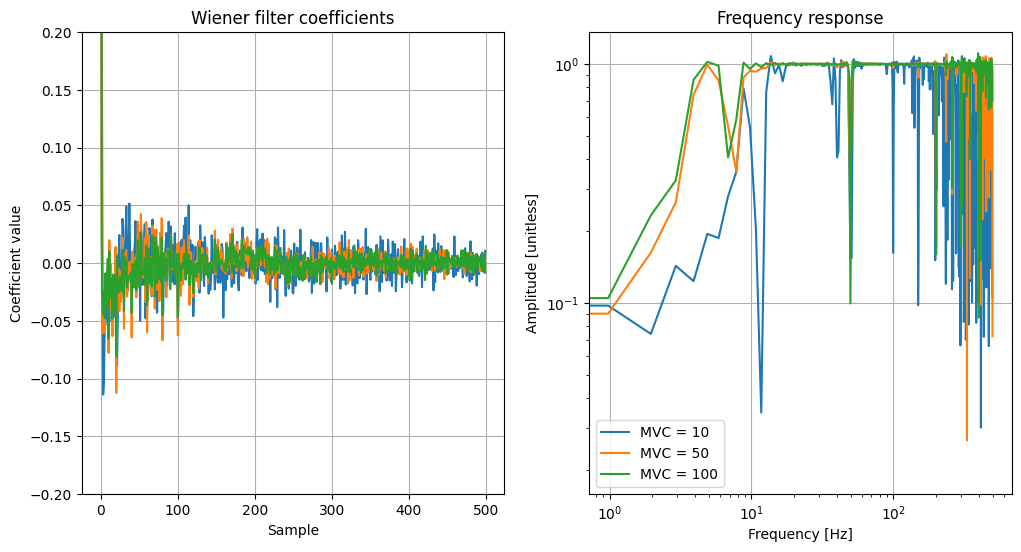
\includegraphics[width=1.0\columnwidth]{images/wiener_filter_response_mvc.png}
	\end{center}
	\caption{The frequency response of a Wiener filter at different levels of MVC. It can be seen that at a lower MVC the filter appears to have a very aggressive frequency response (seen by the large peaks at \SI{10}{\hertz} and higher frequencies) while at higher MVC this response is much less pronounced.}
	\label{fig:wiener_filter_response_mvc}
\end{figure}


\subsubsection{Adaptive filter}
The functioning of an LMS filter has been described in the theory section \ref{sec:filters_theory}. An LMS filter has two properties that determine its behaviour: The filter length and the convergence coefficient. To determine the best combination of these parameters when applied to sEMG signals a range of different values was tested. The results can be found in Figure~\ref{fig:lms_filter_windowsize}. For the measurement section (\ref{sec:measurements}) an LMS filter with length 500 and convergence value of 0.1 will be used.

\begin{figure}[h!t]
	\begin{center}
		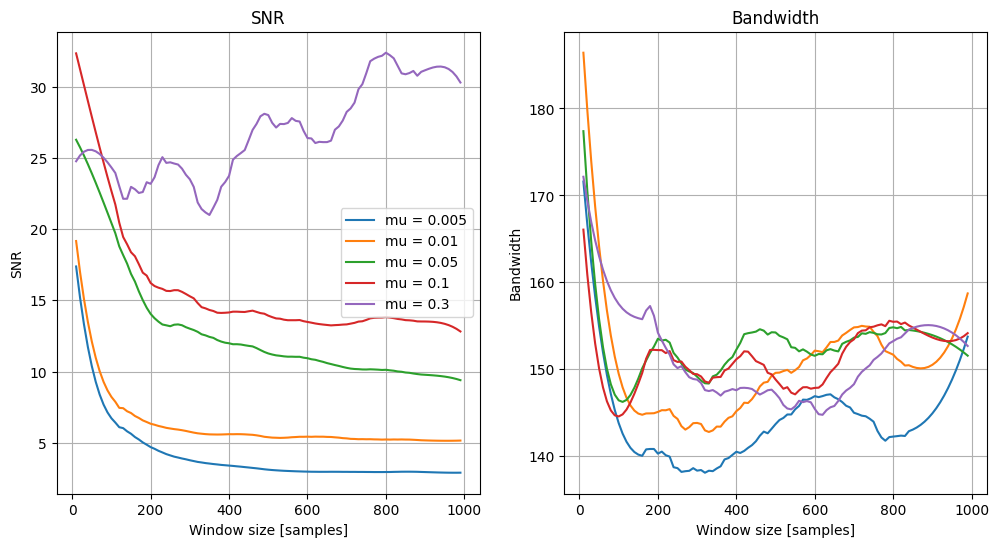
\includegraphics[width=1.0\columnwidth]{images/lms_filter_windowsize.png}
	\end{center}
	\caption{SNR and bandwidth of an adaptive LMS filter using different combinations of filter length and convergence value. It should be noted that each signal has been smoothed using a Savitzky-Golay filter with a window length of 31 and a polynomial order of 3. This is done to make the difference in performance between different convergence values clearer as without filtering the signals have a larger deviation that makes the lines unreadable. A higher convergence value seems to result in a better SNR. Furthermore it seems that increasing window length results to lower SNR (except for the convergence value of 0.3), but to slightly higher bandwidth. A convergence value of 0.1 with a filter length of 500 was chosen as this yields a good middle ground between SNR and bandwidth}
	\label{fig:lms_filter_windowsize}
\end{figure}


\subsection{Results}
A property that might be of interest is each filters performance in different levels of Maximum Voluntary Contraction (MVC). This allows for insight into how well each filter functions in different levels of signal compared to the environment noise. This was realized by keeping the noise constant, but scaling the signal to different levels (from 1-\SI{100}{\percent}) to simulate different levels of MVC. The SNR of the filtered signal and filtered noise was divided by the reference SNR (SNR of input signal and input noise) to be able to draw a clear conclusion about the filters performance. This has as effect that the unfiltered signal results in a horizontal line with the value of 1 as can be seen in \ref{fig:filter_snr_mvc}.

\begin{figure}[h!t]
	\begin{center}
		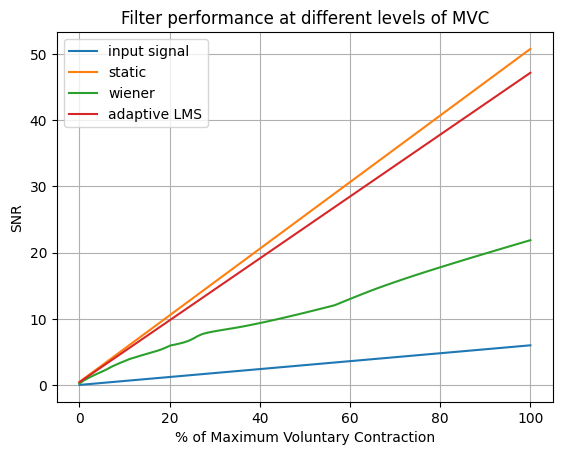
\includegraphics[width=0.7\columnwidth]{images/filter_snr_mvc.png}
	\end{center}
	\caption{The normalized SNR of each filter for different levels of MVC (filter SNR divided by unfiltered signal SNR). It can be seen that there is no relation between the static filters performance and the degree of contraction. An interesting observation can be made about the Wiener filter and the adaptive filter as they seems to perform better at lower MVC. This could be explained by the fact that if noise makes up a larger portion of the signal it might be 'easier' to find a set of filter coefficients that filter a larger portion of noise away. If a few frequencies in the noise are orders of magnitudes larger than those frequencies in the signal, a filter that removes that frequency will impact the noise much more than the signal which results in a higher SNR. For the adaptive filter it may also play a role that the sample on which this is tested was only 2000 samples long which may not have been enough to converge to an approximation of the optimal coefficients. It can also be seen that the SNR of the Wiener filter is much lower than the numbers presented in Figure~\ref{fig:wiener_filter_length}, this may be caused because the plots shown in Figure~\ref{fig:wiener_filter_length} have been smoothed to reflect general behaviour. Without this smoothing, the plot in Figure~\ref{fig:wiener_filter_length} has a large deviation and it is possible that this specific filter length was not great for this specific signal but, given a larger data set, will approximately follow the results presented in Figure~\ref{fig:wiener_filter_length}.}
	\label{fig:filter_snr_mvc}
\end{figure}

Again, the bandwidth was calculated for different filters and at different levels of MVC. The results can be seen in Figure~\ref{fig:filter_bw_mvc}.

\begin{figure}[h!t]
	\begin{center}
		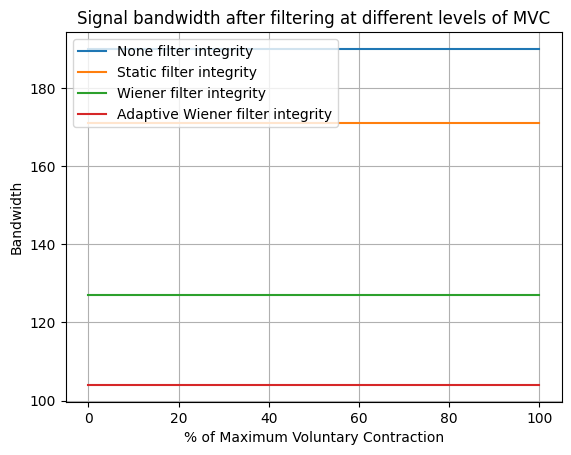
\includegraphics[width=0.7\columnwidth]{images/filter_bw_mvc.png}
	\end{center}
	\caption{The bandwidth of each filter for different levels of MVC. It can be seen that there is no relation between a filters performance and the degree of contraction for the static and adaptive filter. The static filter performs as expected as it removes the same frequency components regardless of the amplitude of the signal. The Wiener filter seems to have larger bandwidth at higher MVC. This can logically be explained by the fact that the optimal filter uses the statistical spectral properties of the entire signal sample, but in situations of low MVC may not result in good filtering on subsets of the signal. The adaptive filter does not have this problem as it can adjust the filter terms to also accurately filter subsets of the data. }
	\label{fig:filter_bw_mvc}
\end{figure}

For bandwidth holds that the metric is independent of degree of muscle contraction as seen in Figures~\ref{fig:filter_bw_mvc} and for SNR this holds except for the non-static adaptive LMS filter as seen in Figure~\ref{fig:filter_snr_mvc}
Figure~\ref{fig:filter_snr_mvc} shows that the best signal to noise ratio is achieved using a Wiener filter, but this filter also has the worst bandwidth performance as seen in Figure~\ref{fig:filter_bw_mvc}. 

\section{Envelope estimation}
\subsection{Comparison metrics}
There are two separate metrics that need to be measured when comparing envelope estimation techniques. The first one is how 'fast' a techniques is, and the second is how 'good' the technique is. The first metric gives information about how much the 'detected' signal lags behind the 'true' signal. The second metric is the quality of the envelope estimate when accounting for the lag.

The lag is detected by calculating the cross-correlation between the true signal and the envelope estimate. Cross-correlation is a metric that determines the similarity between two signals as a function of displacement of one signal relative to another \cite{wiki:cross_correlation}. Since the 'true' signal and the estimated signal are most similar when their displacement equals the lag, a detectable peak is formed in the cross correlation function. The left subplot in Figure~\ref{fig:envelope_estimation_method} displays a 'true' signal (measured force), and a simulated estimation of this signal (estimated force) that lags behind the true signal. The cross-correlation is also plotted that has a peak at \SI{100}{\milli\second}, which is the exact amount of lag between the two signals. The right subplot shows the two signals where the estimated signal has shifted to account for the lag. 

The error can be determined by subtracting the true signal from the estimated signal, and the root-mean-square-error can be calculated. 

\begin{figure}[h!t]
	\begin{center}
		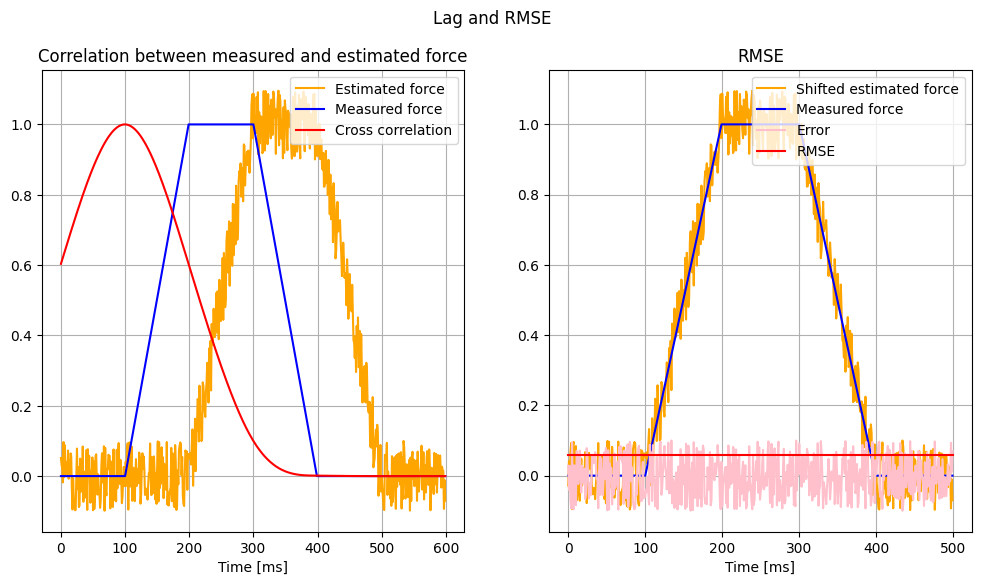
\includegraphics[width=1.0\columnwidth]{images/envelope_estimation_method.png}
	\end{center}
	\caption{Illustration of method for judging envelope estimation}
	\label{fig:envelope_estimation_method}
\end{figure}

An input signal was generated to be Gaussian white noise since it has signal properties close to that of an sEMG signal, and is multiplied with a modulation that can be seen in the left subplot of Figure~\ref{fig:envelope_detection}. The envelope detection techniques are applied onto the input signal and the results are plotted in the right subplot of Figure~\ref{fig:envelope_detection}.

\begin{figure}[h!t]
	\begin{center}
		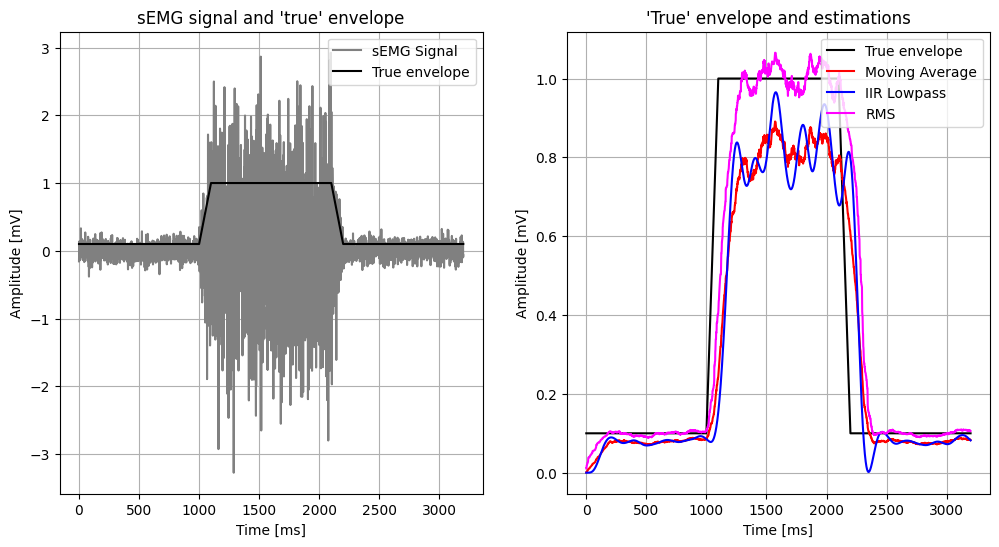
\includegraphics[width=1.0\columnwidth]{images/envelope_detection.png}
	\end{center}
	\caption{Left: Input signal and 'true' envelope'. Right: Envelope detection using different techniques to illustrate difference in behaviour}
	\label{fig:envelope_detection}
\end{figure}

\subsection{Method}
\subsubsection{IIR lowpass filter}
A Butterworth filter was used to construct an IIR lowpass filter. The performance of such a lowpass filter is defined by its $f_\text{cut}$ and the number of filter coefficients (or the filter order). The highest frequency that the envelope should be able to produce is the frequency by which one can contract and relax the measured muscle. It was empirically determined that the maximum frequency for switching between total relaxation and maximum voluntary contraction and back was around \SI{5}{\hertz} and thus the $f_\text{cut}$ was varied from \SI{1}{\hertz}-\SI{9}{\hertz}. The filter length was varied from 2-8 because the minimum possible filter length is 2 (a single filter coefficient provides no filtering, just scaling the signal with a constant), and a filter length >8 resulted in unstable behaviour. A plot of the frequency response of the IIR Butterworth filter can be seen in Figure~\ref{fig:iir_frequencyresponse_coefficients}. The filters are achieved as a numerator/denominator sequence. Since the purpose of this filter is real-time envelope detection, it was applied using scipy's lfilter since as that is causal forward-in-time filtering only.


\begin{figure}[h!t]
	\begin{center}
		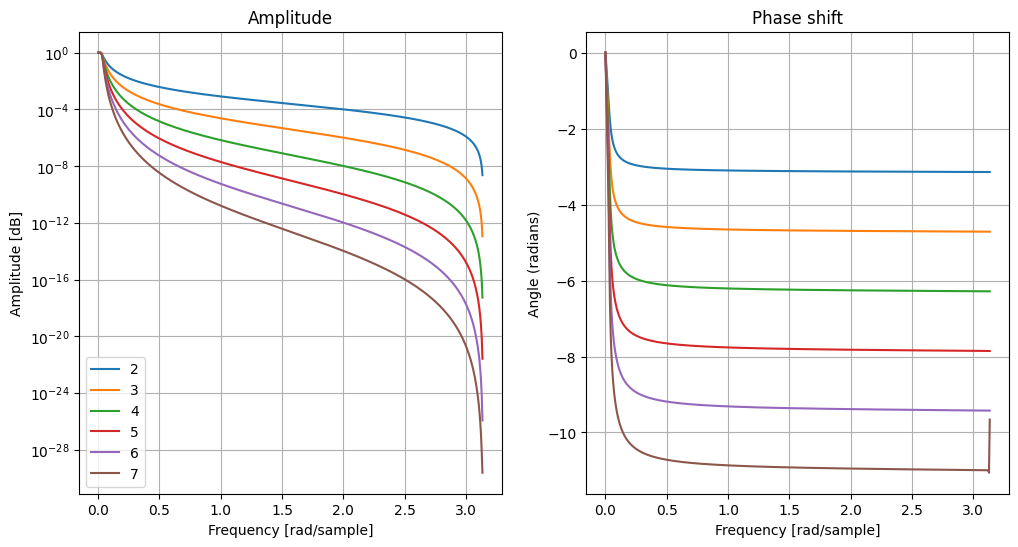
\includegraphics[width=1.0\columnwidth]{images/iir_frequencyresponse_coefficients.png}
	\end{center}
	\caption{Frequency response of IIR Butterworth filter of different order. The $f_\text{cut}$ was set to 5Hz.}
	\label{fig:iir_frequencyresponse_coefficients}
\end{figure}

\subsubsection{Moving average}
The moving average filter only depends on the length of the filter, Figure~\ref{fig:movingaverage_frequencyresponse_coefficients} depicts the frequency behaviour of the moving average filter of different lengths. The range of values that are tested is chosen arbitrarily, but large enough to cover general use cases.

\begin{figure}[h!t]
	\begin{center}
		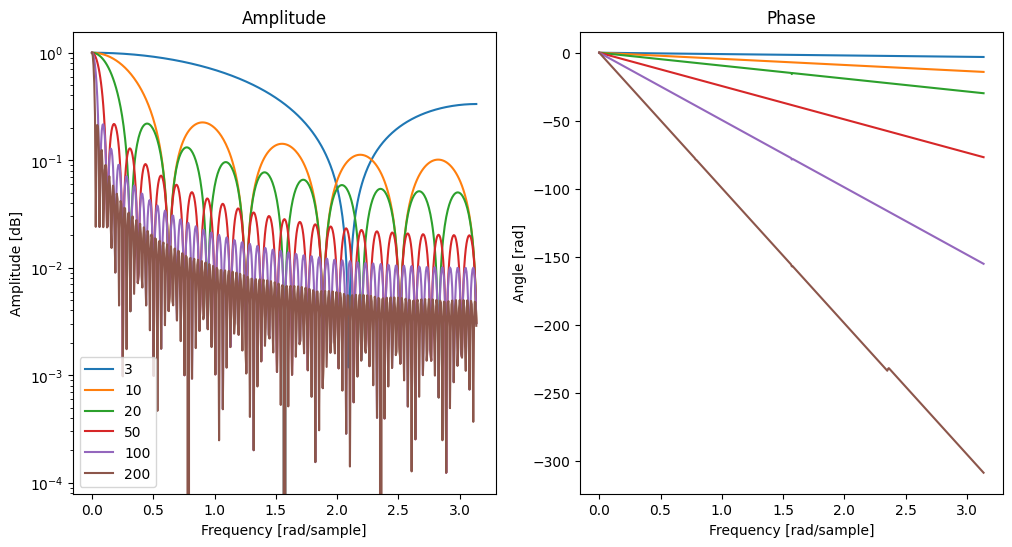
\includegraphics[width=1.0\columnwidth]{images/movingaverage_frequencyresponse_coefficients.png}
	\end{center}
	\caption{Frequency response of moving average filter of different lengths. The coefficients of the moving average filters are 1/length of filter.}
	\label{fig:movingaverage_frequencyresponse_coefficients}
\end{figure}

\subsubsection{Root mean square}
Similar to the moving average filter, the behaviour of the RMS filter is solely determined by the length of the filter. The same range of filter lengths was chosen as for the moving average filter so that the performance could be directly plotted against each other.

\subsection{Results}
To properly evaluate the performance of the envelope detection techniques each method has been tested individually across the range of variables that were described in the previous method section and plotted against the resulting lag and error. 

The graph describing the performance of the IIR Butterworth filter can be seen in Figure~\ref{fig:lagerror_iir}. The graph describing the performance of the moving average filter and the RMS filter can be seen in Figure~\ref{fig:lagerror_RMS_MA}.

\begin{figure}[h!t]
	\begin{center}
		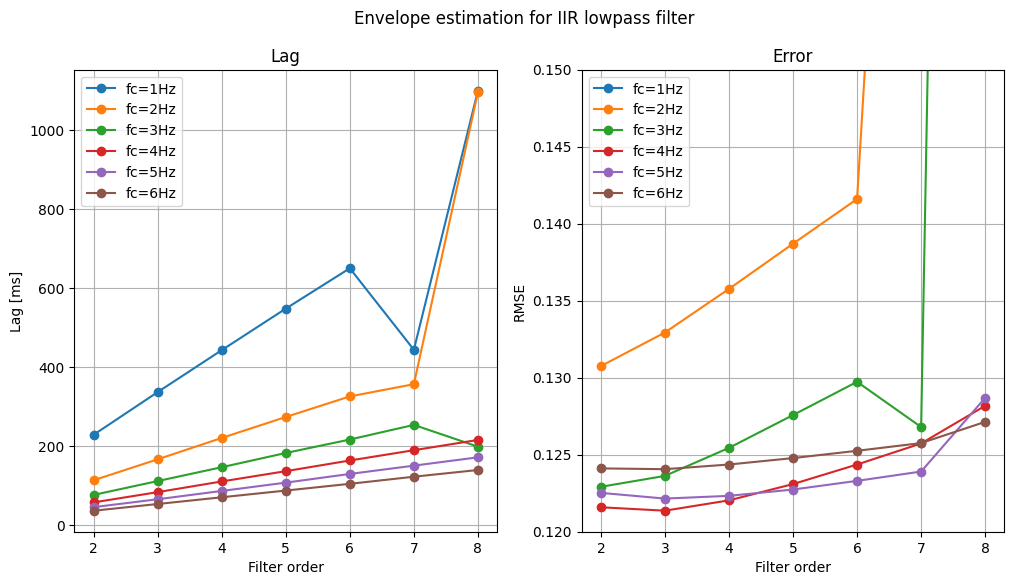
\includegraphics[width=1.0\columnwidth]{images/lagerror_iirfilter.png}
	\end{center}
	\caption{Lag and error of an IIR Butterworth filter for different cut-off frequencies and filter lengths. Note that filters with a lower $f_\text{cut}$ and high number of filter coefficients become unstable which can be seen in the error-graph for cut-off frequencies \SI{1}{\hertz}-\SI{3}{\hertz}. Additionally, the error in these graphs are all below 0.125. This is caused by the fact that the modulation is between 0 and 1, the error is <1 and the squared error is smaller still. So not the error value, but the \textit{relation between} error values of different methods is the truly useful information here.}
	\label{fig:lagerror_iir}
\end{figure}

\begin{figure}[h!t]
	\begin{center}
		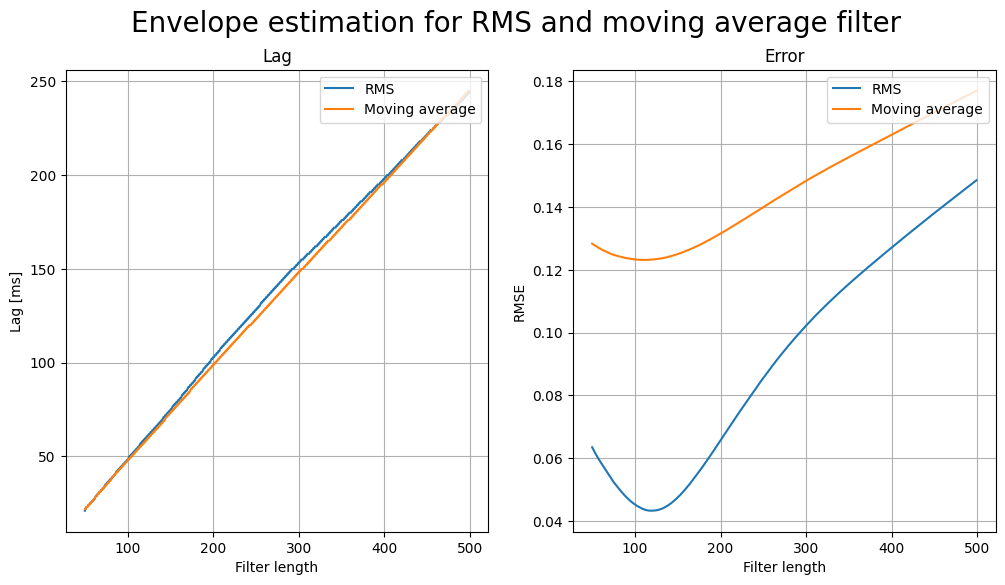
\includegraphics[width=1.0\columnwidth]{images/lagerror_rms_and_MA_filter.png}
	\end{center}
	\caption{Lag and error of RMS filter and moving average filter for different filter lengths}
	\label{fig:lagerror_RMS_MA}
\end{figure}

From Figure~\ref{fig:lagerror_iir} it can be seen that an IIR LP Butterworth filter of length 3 and $f_\text{cut}$ of \SI{4}{\hertz} results in the lowest error. A filter with $f_\text{cut}$ of \SI{6}{\hertz} has the lowest lag but this is only marginally less than a $f_\text{cut}$ of \SI{4}{\hertz}. For this reason an IIR LP Butterworth filter of length 3 and $f_\text{cut}$ of \SI{4}{\hertz} is used in the the measurement section (\ref{sec:measurements}).

From Figure~\ref{fig:lagerror_RMS_MA} it can be seen that moving average and RMS methods have similar lag, and the lag has a linear relation to the filter length. In the same figure it can also be seen that the error reaches a minimum at a filter length of 120. For this reason both the RMS and moving average method are applied with a filter length of 120. The Figure also shows that the error increases with more filter terms which may seem counter-intuitive. A possible explanation for this is that filters with more filter coefficients can achieve a higher transition bandwidth. As a result, the envelope may be detected through a sets of frequencies that does not accurately represent the applied force. Shorter filters have smaller transition bandwidth and thus a 'smoother' frequency range is used to construct the envelope.

\section{Force estimation}\label{section:force_estimation}
The measured sEMG signals from antagonistic muscles needs to be combined to form an estimate of the exerted force. Since this calculation is done in a consistent way throughout all measurements this section serves purely to provide some insight into the method of calculation.

The previous step of envelope estimation is used to get a measure of muscle activation. Since muscle activation leads to muscle contraction and exerted force around a joint is the difference between how much antagonistic contract \cite{human_robotics} it becomes possible to determine the force from sEMG. To correlate the difference in muscle contraction from antagonistic muscles (such as biceps and triceps) to the exerted force, the muscle contraction needs to be scaled. As previously mentioned, a linear relation between sEMG and force will be assumed \cite{adaptive_filter_dry_electrode} \cite{interpreting_muscle_function_from_emg}. In Figure~\ref{fig:force_simulation} it is shown how the exerted force is estimated from simulated bicep and triceps sEMG. 

\begin{figure}[h!t]
	\begin{center}
		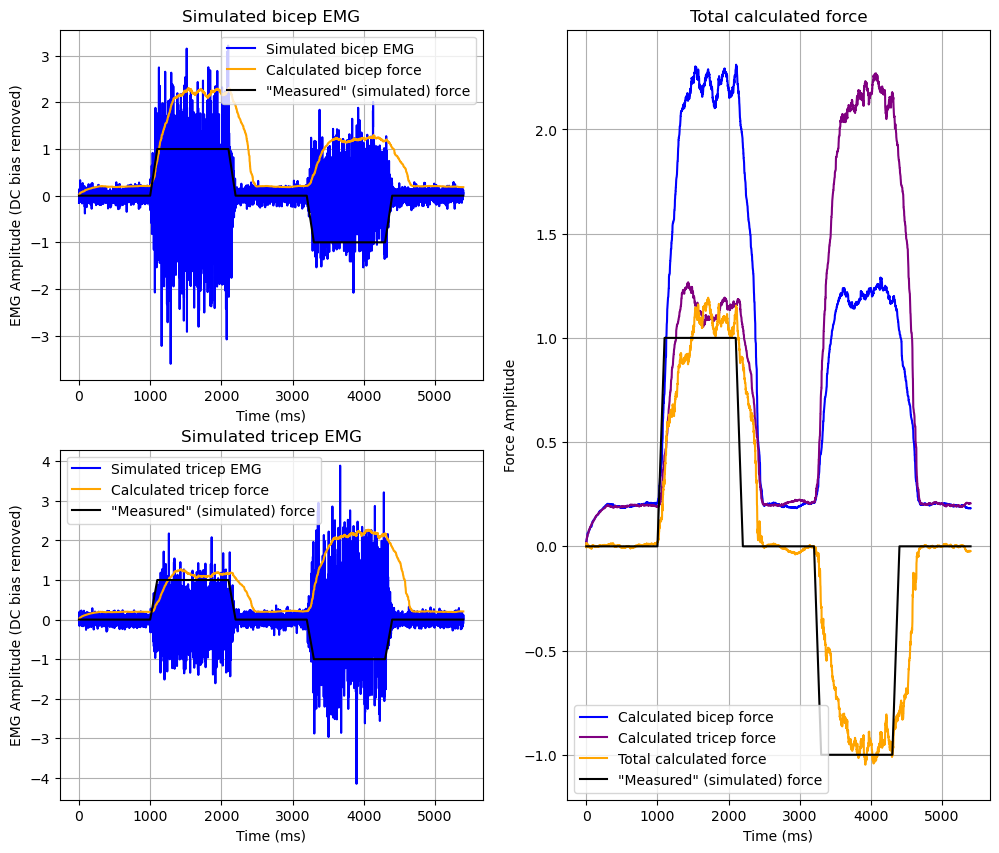
\includegraphics[width=1.0\columnwidth]{images/force_simulation.png}
	\end{center}
	\caption{Process of estimating force from simulated sEMG (random Gaussian noise). The bicep envelope is calculated at the top, notice how during downwards force exertion the bicep still activates but to a lesser degree than during upwards force exertion. The same holds for the triceps in the bottom figure. The subplot on the right shows the envelope of the bicep, triceps, the difference between these two (identical to estimated force assuming linear scaling with factor 1), and the 'measured' force .}
	\label{fig:force_simulation}
\end{figure}

\section{Conclusion}
In this chapter different filtering and envelope detection methods were compared. For each method, different variations of parameters were tested to determine the most optimal solution for each option.
From the presented simulations the following expectations are made:
\begin{itemize}
    \item The static filter performs the best in terms of SNR, but in terms of bandwidth performs worse than other filters. The unfiltered signal yields the largest bandwidth but the lowest SNR. From this it is expected that if a high SNR results in a more accurate force estimation from sEMG that the static filter will perform best in force estimation as long as the MVC is large as seen in Figure~\ref{fig:filter_snr_mvc}, but if MVC is small then the adaptive LMS filter is expected to perform best.If bandwidth is the most important property for estimating force from sEMG it is expected that unfiltered signals perform the best, closely followed by the adaptive LMS filter and Wiener filter.
    \item The RMS envelope detection method results in the smallest error compared to moving average and IIR Low-pass filter for the determined filter parameters. In terms of lag the RMS envelope detection performs about the same as the moving average envelope detection, and both of these are expected to result in less lag than IIR LP filter.
\end{itemize}
